\documentclass[11pt,a4paper]{article}
\usepackage[top=1.4cm,bottom=1.4cm,left=1.8cm,right=1.8cm]{geometry}
\usepackage{graphicx}
\usepackage{booktabs}
\usepackage{enumitem}
\usepackage{parskip}
\usepackage{titlesec}
\usepackage{amsmath}
\usepackage{amssymb}
\usepackage{grffile}
\usepackage[hidelinks]{hyperref}

\titleformat{\section}[block]{\bfseries\normalsize}{}{0em}{}%
  [\vspace{-0.4em}\rule{\linewidth}{0.4pt}]
\titlespacing{\section}{0pt}{7pt}{4pt}
\setlist[itemize]{noitemsep,topsep=1pt,leftmargin=*}

\begin{document}

\begin{center}
  {\Large\bfseries Planetary Orbit Visualisation --- WebGL 2.0}\\[4pt]
  Abdullah Khan Sherwani\quad|\quad Computer Graphics
\end{center}

%------------------------------------------------------------------------------
\section{Project Direction}

\textbf{Scene Rendering System} --- a visually rich 3-D space scene with
multiple celestial bodies, physically motivated lighting, and interactive camera
control.

%------------------------------------------------------------------------------
\section{Idea Description}

The application renders a gas giant and its icy moon in real time using a
hand-written WebGL 2.0 / GLSL ES 3.00 pipeline (no game engine).
The planet rotates on a tilted axis and is encircled by a semi-transparent ring
system rendered as an alpha cutout.
The moon orbits hierarchically and the two bodies exchange analytical shadows:
the planet eclipses the moon on the far side and the moon casts a transit shadow
dot on the planet when it crosses the sun.
The user can orbit the scene freely with mouse/touch and scroll to zoom, and can
toggle camera focus between the planet and the moon with a key press.

%------------------------------------------------------------------------------
\section{Baseline Techniques}

\smallskip
\begin{tabular}{@{}p{5.8cm}p{1.6cm}p{7.6cm}@{}}
\toprule
Technique & Applies & Notes \\
\midrule
Phong  & Yes & \\
Material shininess \& reflectance    & Yes & \\
Diffuse texture maps                 & Yes & \\
Specular maps                        & Yes & \\
Per-fragment lighting                & Yes & \\
Directional light                    & Yes & \\
Point lights with attenuation        & No
  & Space scene has a single light source (the sun); no artificial point lights exist \\
Spotlights with smooth falloff       & No
  & No cone-constrained lights applicable to this scene \\
Multiple light accumulation          & No
  & Only one light source (directional sun); multi-light accumulation does not apply \\
GLSL uniforms \& normal matrix       & Yes & \\
\bottomrule
\end{tabular}

%------------------------------------------------------------------------------
\section{Advanced Techniques}

\smallskip
\begin{tabular}{@{}p{4.2cm}p{1.2cm}p{9.6cm}@{}}
\toprule
Technique & Effort & Implementation \\
\midrule
Bloom & 4/5
  & Bright-region extract pass $\to$ 6-pass separable Gaussian
    blur (ping-pong FBOs) $\to$ additive composite to screen \\
Environment Mapping & 3/5
  & Star-field cubemap sampled via \texttt{reflect(-V,N)}
    per-fragment; contribution scaled by surface specular coefficient \\
Fog & 2/5
  & Exponential deep-space fog; blends fragments toward
    a void colour with camera distance \\
Gamma Correction & 2/5
  & Linear $\to$ gamma via \texttt{pow(max(col,0), vec3(1/2.2))}
    at end of shader \\
\midrule
\textbf{Combined} & \textbf{11/10}
  & Requirement: $\geq 6/10$, at least one technique $\geq 3$ \quad $\checkmark$ \\
\bottomrule
\end{tabular}

\smallskip
{\small\textit{Note: the selection of advanced techniques may be adjusted during
implementation depending on feasibility and scope.}}

%------------------------------------------------------------------------------
\section{Inspiration Images}

\begin{figure}[h]
\centering
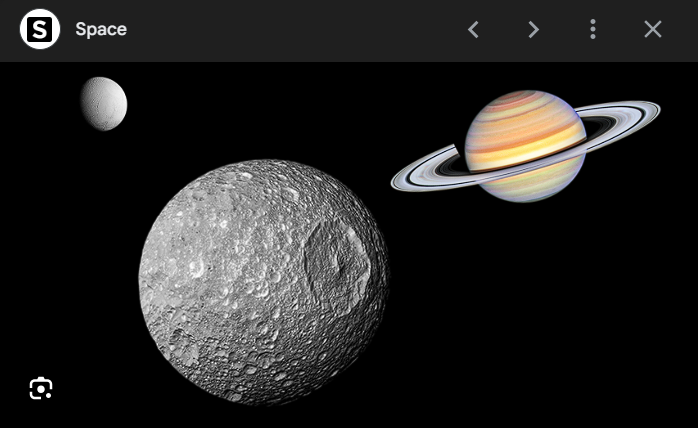
\includegraphics[width=0.32\linewidth]{../Assets/Reference Pictures/image.png}\hfill
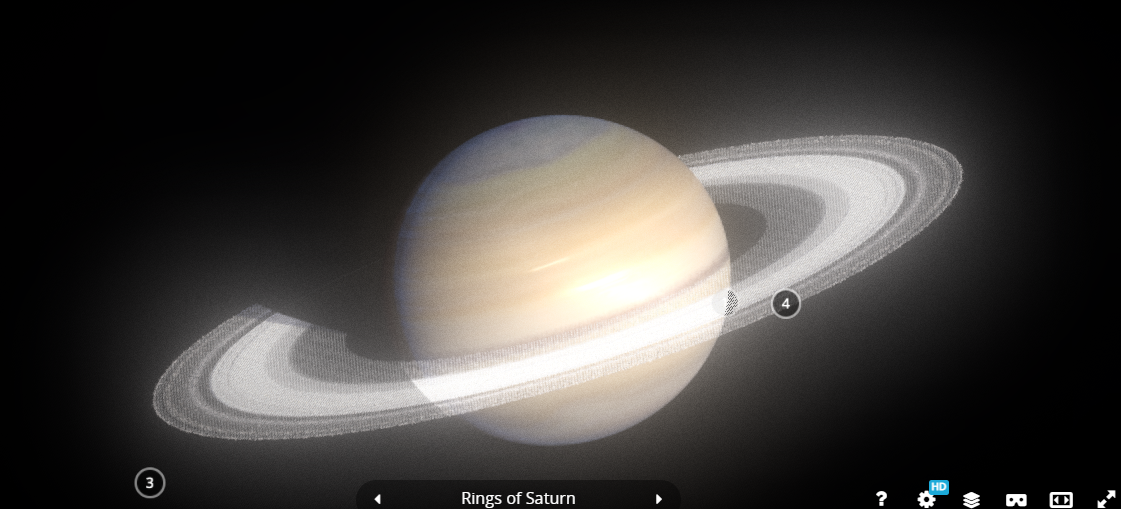
\includegraphics[width=0.32\linewidth]{../Assets/Reference Pictures/Screenshot 2026-04-27 144757.png}\hfill
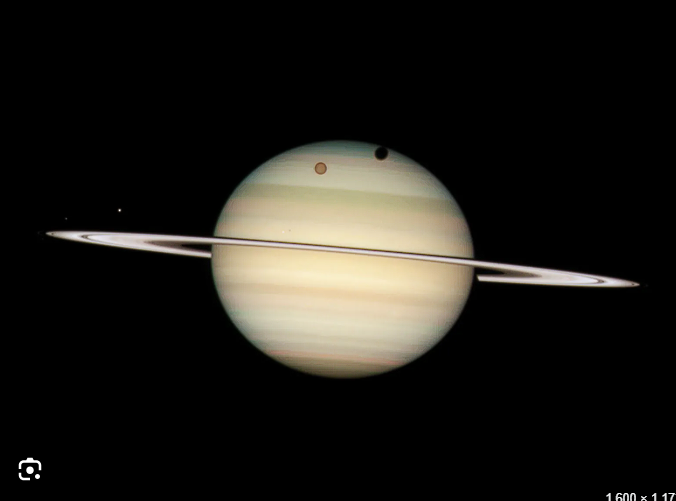
\includegraphics[width=0.32\linewidth]{../Assets/Reference Pictures/Screenshot 2026-04-28 182947.png}
\\[4pt]
{\small
  \textit{Left:} Reference render 1.\quad
  \textit{Centre:} Reference render 2.\quad
  \textit{Right:} Reference render 3.}
\end{figure}

%------------------------------------------------------------------------------
\section{Implementation Plan}

\begin{itemize}
  \item \textbf{Step 1} --- WebGL 2.0 context, VAO/VBO pipeline, per-fragment
        Phong shader with directional sun and 8K texture mapping.
  \item \textbf{Step 2} --- GLB asset loading; scene-unit
        normalisation; hierarchical orbit transform with axial tilt and rings.
  \item \textbf{Step 3} --- Cubemap skybox and environment mapping
        (per-fragment reflection vector sampling).
  \item \textbf{Step 4} --- Bloom post-process (FBO pipeline); exponential fog;
        gamma correction.
  \item \textbf{Step 5} --- Analytical inter-body shadows (ray-sphere test in
        fragment shader); view-toggle camera (planet $\leftrightarrow$ moon).
  \item \textbf{Step 6} --- Polish: ring alpha cutout, anisotropic filtering,
        specular/gloss textures, performance tuning.
\end{itemize}

%------------------------------------------------------------------------------
\section{External Assets}

\smallskip
\begin{tabular}{@{}p{4.4cm}p{6.2cm}p{4.4cm}@{}}
\toprule
Asset & Source & Licence \\
\midrule
Planet \& moon 3-D models
  & Sketchfab (BlendSwap mirror)
  & CC-BY \\
8K planet, ring \& sun textures
  & \href{https://www.solarsystemscope.com/textures/}{solarsystemscope.com}
  & CC-BY \\
Milky Way starmap cubemap
  & NASA / STScI --- Gaia DR2 all-sky image
  & Public domain \\
\texttt{gl-matrix} (math library)
  & \href{https://npmjs.com/package/gl-matrix}{npmjs.com}
  & MIT \\
\bottomrule
\end{tabular}

\end{document}
